\chapter{Monster Black Holes in Massive Galaxies}
\label{ch:msigma}

A precise measurement of the log-slope of the $M_{\rm BH} - \sigma_*$ correlation is important 
to constrain theoretical models of AGN feedback. 
For example, energy driven outflows are expected to produce a scaling of $M_{\rm BH} \propto \sigma_*^5$, 
whereas momentum driven outflows should result into a shallower $M_{\rm BH} \propto \sigma_*^4$ relation 
\citep{silkrees1998,fabian1999}. 
Since the $M_{\rm BH} - \sigma_*$ correlation was presented for the first time by \citet{ferraresemerritt2000}
and \citet{gebhardt2000}, 
there has been an ongoing, lively debate about its log-slope, 
whose estimates differed by up to a few standard deviations 
depending on the choice of galaxy sample, the method used to measure the velocity dispersion,
the assumed uncertainty associated with the velocity dispersion, 
and the linear regression algorithm (e.g.~\citealt{tremaine2002}). \\ 

Recent measurements of SMBH masses in Central Cluster Galaxies (CCGs)
have added new data points at the high-mass end of the 
$M_{\rm BH} - \sigma_*$ diagram \citep{mcconnell2011,mcconnell2012}, 
which appear to be outlying (``over-massive'') with respect to the observed correlation. 
\citet{volontericiotti2013} explained the presence of over-massive black holes in CCGs 
(they included in this definition either central dominant galaxies or brightest cluster galaxies) 
as a natural consequence of the fact that these galaxies have experienced more dry mergers 
than any other early-type galaxy (see also \citealt{kormendyho2013}). 
Their semi-analytical models are based on the idea that parabolic dissipationless dry mergers 
increase a galaxy's mass, luminosity and effective radius, 
but do not significantly change its velocity dispersion (e.g.~\citealt{ciotti2007}). 
Let an elliptical galaxy be a non rotating, isotropic and virialized spheroidal system 
with stellar mass $M_{*}$ and gas mass $M_{\rm g} = \alpha M_{*}$. 
The total energy $E$ of this galaxy is the sum of its total kinetic energy $K$ and its total gravitational energy $W$. 
The total kinetic energy is given by the sum of the stellar kinetic energy $K_*$ and the gas internal energy $K_{\rm g}$, 
therefore the total energy can be expressed as:
\begin{equation}
E = K_* + K_{\rm g} + W \ .
\end{equation}
The stellar kinetic energy is 
\begin{equation}
K_* = \frac{3}{2} M_* \sigma_*^2 \ ,
\end{equation}
where $\sigma_*$ is the stellar velocity dispersion. \\
The gas internal energy is defined as 
\begin{equation}
K_{\rm g} = \frac{3}{2} \frac{k_{\rm B}}{\bar{m} } \int_{\mathcal{V}} \rho_{\rm g} T d\mathcal{V} \ ,
\end{equation}
where $k_{\rm B}$ is the Boltzmann constant, $\bar{m}$ is the gas mean molecular mass, and 
$\rho_{\rm g}$ and $T$ are the density spatial distribution and the temperature of the gas, respectively, 
within the galaxy's volume $\mathcal{V}$. \\
The total gravitational energy is defined as 
\begin{equation}
W = \frac{1}{2} \int_{\mathcal{V}} (\rho_* + \rho_{\rm g}) (\phi_* + \phi_{\rm g}) d\mathcal{V} \ , 
\end{equation}
where $\rho_*$ is the density spatial distribution of stars, 
and $\phi_*$ and $\phi_{\rm g}$ indicate the gravitational potential of stars and gas, respectively. \\
Under the assumption of gas in equilibrium in the total gravitational field, 
from the Jeans and hydrostatic equations one has that $T = \bar{m} \sigma_*^2 / k_{\rm B}$ and thus 
\begin{equation}
K_{\rm g} = \alpha K_* \ .
\end{equation}
Assuming also that the spatial distribution of gas is proportional to that of stars (i.e.~$\rho_{\rm g} = \alpha \rho_*$ 
and $\phi_{\rm g} = \alpha \phi_*$), 
the total gravitational energy can be written as 
\begin{equation}
W = \frac{1}{2} (1+\alpha)^2 \int_{\mathcal{V}} \rho_* \phi_* d\mathcal{V} = (1+\alpha)^2 W_* \ ,
\end{equation}
where $W_*$ is the gravitational energy of the stellar component only. \\
From the virial theorem (i.e.~$E = K+W = W/2 = -2K$), the galaxy's total energy can be expressed as 
\begin{equation}
E = \frac{1}{2} (1+\alpha)^2 W_* = - (1+\alpha) K_* \ .
\end{equation}
We now consider the parabolic dissipationless merger of two galaxies (with stellar masses $M_{*1}$ and $M_{*2}$,
and total energies $E_1$ and $E_2$), 
i.e.~a merger where both the total energy and the total mass are conserved, 
and no gas is converted into stars. \\
The gas fraction $\alpha$ of the merger remnant is by definition
\begin{equation}
\alpha = \frac{M_{\rm g}}{M_*} = \frac{M_{\rm g1} + M_{\rm g2}}{M_{*1}+M_{*2}} \ ,
\end{equation}
where the nomenclature is self-explicative. \\
By imposing the conservation of total energy, we get 
\begin{equation*}
E = E_1 + E_2 
\end{equation*}
\begin{equation*}
-(1+\alpha) \frac{3}{2} M_* \sigma_*^2 = -(1+\alpha_1) \frac{3}{2} M_{*1} \sigma_{*1}^2 -(1+\alpha_2) \frac{3}{2} M_{*2} \sigma_{*2}^2 \\
\end{equation*}
\begin{equation*}
\bigl[ (1+\alpha_1)M_{*1} + (1+\alpha_2)M_{*2} \bigr ] \sigma_*^2 = (1+\alpha_1)M_{*1}\sigma_{*1}^2 + (1+\alpha_2)M_{*2}\sigma_{*2}^2
\end{equation*}
\begin{equation}
\sigma_*^2 = \frac{(1+\alpha_1)M_{*1}\sigma_{*1}^2 + (1+\alpha_2)M_{*2}\sigma_{*2}^2}{\bigl[ (1+\alpha_1)M_{*1} + (1+\alpha_2)M_{*2} \bigr ]} \ .
\label{eq:sigma*2}
\end{equation}
By defining $c_1 = (1+\alpha_1)M_{*1}/\bigl[ (1+\alpha_1)M_{*1} + (1+\alpha_2)M_{*2} \bigr ]$ 
and $c_2 = (1+\alpha_2)M_{*2}/\bigl[ (1+\alpha_1)M_{*1} + (1+\alpha_2)M_{*2} \bigr ]$, 
Equation \ref{eq:sigma*2} can be simplified as 
\begin{equation}
\sigma_*^2 = c_1 \sigma_{*1}^2 + c_2 \sigma_{*2}^2 \ .
\end{equation}
Finally, since $c_1 + c_2 = 1$, we have that 
\begin{equation}
\min(\sigma_{*1}^2, \sigma_{*2}^2) \leq \sigma_*^2 \leq \max(\sigma_{*1}^2, \sigma_{*2}^2) \ ,
\end{equation}
that is, the velocity dispersion of the merger remnant cannot be larger 
than the maximum velocity dispersion of the progenitor galaxies. 
This conclusion is not true in case of a wet merger or non-parabolic (i.e.~bound) orbits of the progenitors. \\

Whether or not considering the over-massive black holes as an ``exception to the rule'', 
or in other words legitimately excluding them from the linear regression analysis of the $M_{\rm BH} - \sigma_*$ diagram, 
obviously has an impact on the estimate of the log-slope of the correlation. 
Therefore, it is important to test the scenario proposed by \citet{volontericiotti2013} 
with empirical data. \\

The remainder of this Chapter comprises the published version of the paper 
``Overmassive black holes in the $M_{\rm BH} - \sigma$ diagram 
do not belong to over (dry) merged galaxies'' 
by G.~A.~D.~Savorgnan \& A.~W.~Graham,  
as it appears in Volume 446 of \emph{Monthly Notices of the Royal Astronomical Society}. 


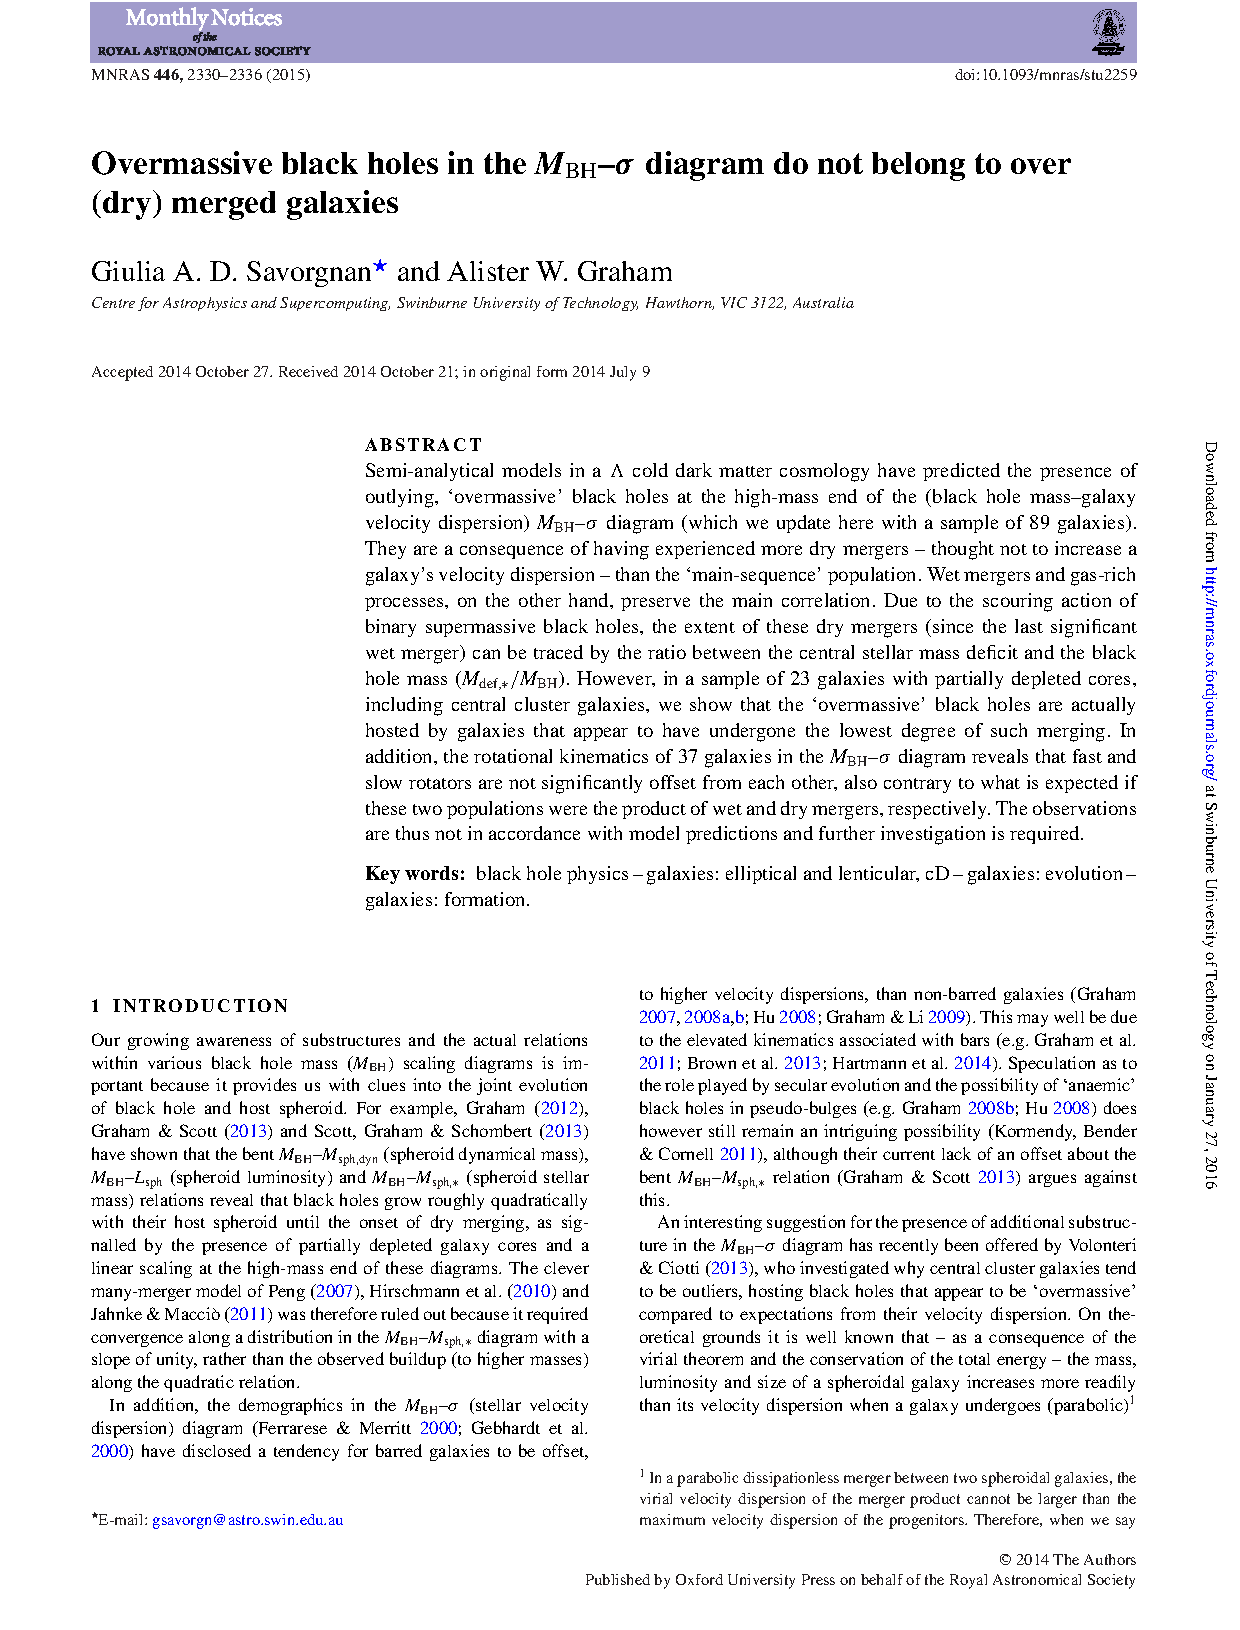
\includepdf[pages={1-7}]{MNRAS2015.pdf}
